\section{Background}

\subsection{ParSplice}
\label{sec:parsplice}

\begin{figure}[t]
  \noindent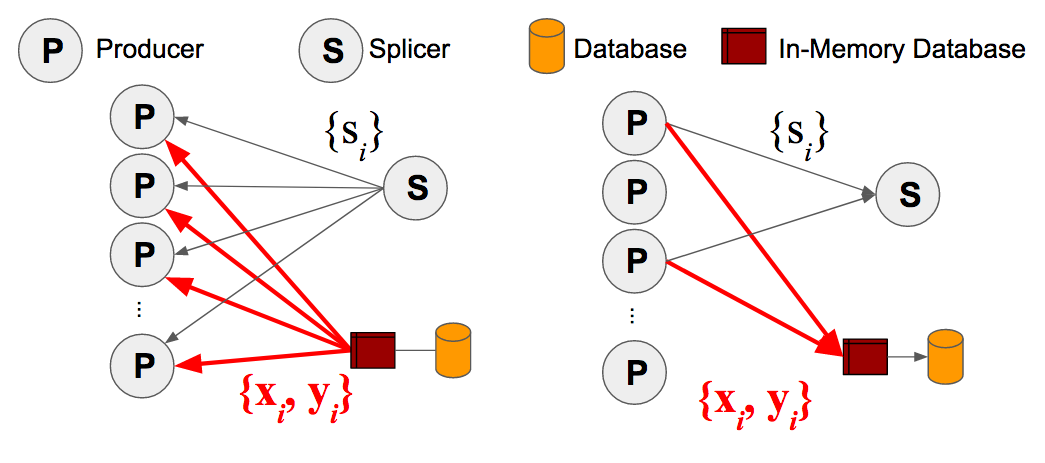
\includegraphics[width=19pc,angle=0]{figures/arch-parsplice.png}\\
  \caption{ParSplice is a ready-heavy HPC application where producers use a
  database for consistency. Replacing the single-node database with HXHIM
  improves performance with load balancing.
  \label{fig:arch-parsplice}}
\end{figure}


ParSplice~\cite{perez:jctc20150parsplice} is a molecular dynamics simulation
developed at LANL. It has 4 phases, as depicted in Figure~\ref{fig:arch-parsplice}:

\begin{enumerate}

  \item splicer (S) tells producers (P) to compute segments for state \(s_i\)

  \item P`s pull initial coordinates \{\(x_i, y_i\)\} from database

  \item a P inserts completed coordinates for segment \(s_i\) into database and
  S broadcasts next segment(s) \(s_j\) 

  \item P`s pull new segment coordinates \{\(x_j, y_j\)\}

\end{enumerate}

The database is single node (LevelDB or BerkeleyDB) with caches in front. Our
goal is to replace this architecture with a distributed key-value store to
solve the immediate sync problems that the ParSplice team is facting. Sliding
in something like MDHIM~\cite{greenberg:hotstorage2015-mdhim} has the added
benefit of enabling load balancing. ParSplice has distinct workload phases and
a well-known keyspace (Figure~\ref{fig:methodology-keyspace}) so its
performance should improve with better load balancing.

\subsection{MDHIM: Key-Value Store for HPC}
\label{sec:hxhim}

\begin{figure}[tb]
  \noindent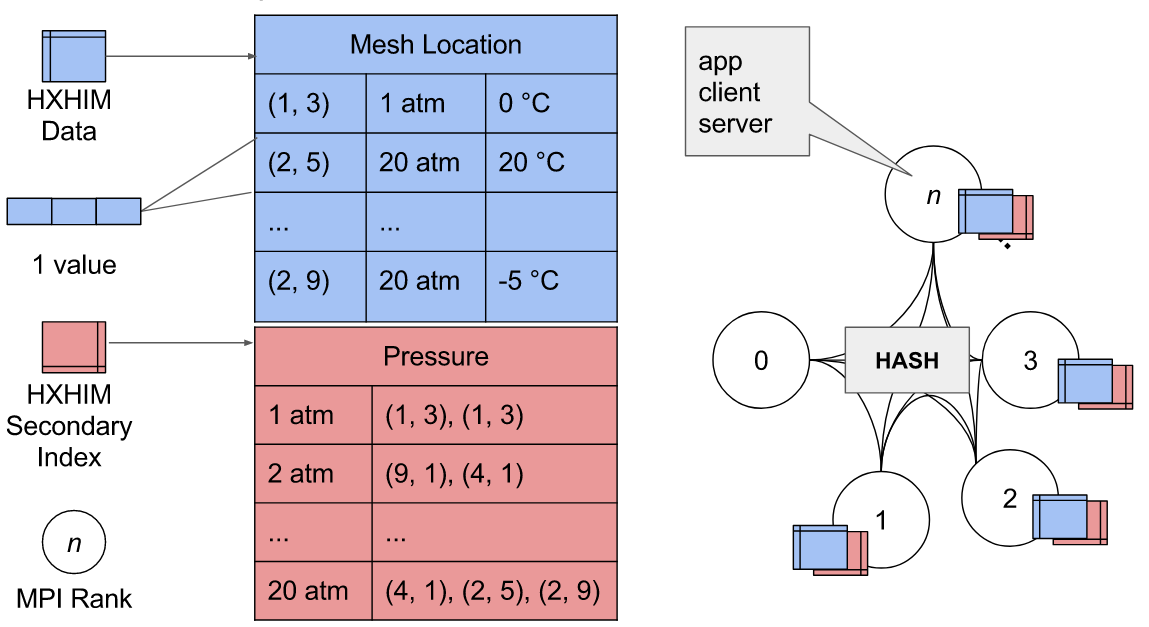
\includegraphics[width=19pc,angle=0]{figures/arch-hxhim.png}\\
  \caption{The MDHIM architecture.}
  \label{fig:arch-hxhim}
\end{figure}

% What is MDHIM
MDHIM is a key-value store designed for HPC architectures and multi-dimensional
data. It is based off MDHIM~\cite{greenberg:hotstorage2015-mdhim}, the
multi-dimensional indexing middleware. Figure~\ref{fig:arch-hxhim} has a crude
sketch of the MDHIM architecture. Each MPI rank has an instance of the
application, which has the client library linked in. An MPI rank can also have
a ``range server", which stores the key-value pairs in a local databse (either
LevelDB or MySQL). Data is located with a consistent hash, which is
configurable.

% What are the indexes?
The primary and secondary indices shown on the right side of
Figure~\ref{fig:arch-hxhim} are views of the data that the range server
manages.  The primary index is the same hash used by the global partitioner.
The secondary index or indices are user-defined tables organized in a different
way from the primary index. The goal of the secondary indices is to speed up
queries that need to aggregate dat ({\it e.g.} find the maximum values). In the
example, the range server and the key in the primary index is located with a
hash of the mesh location. The secondary index is organized by pressure, so
queries asking for a certain atmosphere can be serviced in O\(1\), consisting
of one lookup in the pressure index and one lookup into the primary index.

% Why is it tailored to HPC?
MDHIM tailors its mechanisms and policies to HPC, showing improved performance
over cloud-based key-value stores like Cassandra. It has cursor types for
walking the key-value store, bulk operations for exploiting data locality,
per-job server spawning, and pluggable backends for its local database and
network type (infiniband/RDMA). Its policies are flexible, supporting
customized partitioning strategies and user-defined secondary indices. This
allows the system to choose whether to send load to the client or server.

%\subsection{Comparing Mantle and MDHIM}
%\begin{table*}
%\centering
%\begin{tabular}[tb]{ r | l | l | l | l }
%                       & 
%                       & \multicolumn{1}{c|}{\centering Both} 
%                       & \multicolumn{1}{c|}{\centering Mantle/CephFS}
%                       & \multicolumn{1}{c}{\centering MDHIM}
%                       \\\hline
%  workload   & characteristics     & small/frequent requests  & data access            & data management \\
%             & write-intensive     & partition across cluster & fragment directories*  & NOT IMPLEMENTED \\
%             & read-intensive      & replicate across cluster & copy directories*      & NOT IMPLEMENTED \\\hdashline
%  system     & measure workload    & yes                      & directory temperature  & range server counts \\
%  mechanisms & measure utilization & yes                      & CPU, network, memory   & range server buffer size \\
%             & migrate resources   & almost                   & \texttt{export\_dir()} & \texttt{mdhimB}\{\texttt{Get}, \texttt{Put}\}\texttt{()} \\
%             & partition resources & yes                      & subtrees \& dirfrags   & secondary index, cursor type, bulk operations\\\hdashline
%  migration  & interval            & configurable             & every 10 seconds       & every query \\
%  decisions  & global state        & decentralized decisions  & heartbeats for metrics & NOT IMPLEMENTED \\
%  \multicolumn{5}{c}{}\\
%  \multicolumn{5}{c}{\tiny *Mechanisms implemented in CephFS, not integrated into Mantle}
%\end{tabular}
%\caption{Comparing the design goals and implementatons of Mantle and MDHIM.}
%\label{fig:arch-comparison}
%\end{table*}
%
%% Why are the designed for the same type of workload?
%The ``Both" column of Table~\ref{fig:arch-comparison} shows how Mantle and
%MDHIM have similar designs. The workloads are very similar as the the services
%respond to small and frequent requests, which results in hot spots and flash
%crowds. As a result, popularity of the data, not the size, drives distribution
%in both systems. Both workloads also have data locality so the systems have
%mechanisms for leveraging requests with similar semantic meaning.  Finally, the
%overall design of both systems is decentralized meaning that there is no
%centralized scheduler and each server has an inconsistent global view.
%
%% What are the challenges?
%Despite the similarities, integrating the Mantle API with MDHIM has both design
%and technical challenges. Mantle is reactive to the workload as opposed to
%MDHIM migrations, which are triggered based on the request type. As a result,
%Mantle has functionality for exchanging server utilization (CPU, network,
%memory) and workload (tracks request types). MDHIM 
%
%
%%This paper takes the API and load balancers designed in
%%Mantle~\cite{sevilla:sc15-mantle}, the programmabile file system metadata load
%%balancer for Ceph, and applies them to
%%MDHIM~\cite{greenberg:hotstorage2015-mdhim}, the distributed key-value store
%%designed for HPC.
%
%
%
%Results should show, In order from most likely to least likely:
%
%\begin{enumerate}
%
%  \item HPC key-value store workloads are structured (because they are mostly
%  workflows and simulations) that their job phases can be learned and exploited
%  using dynamic load balancing policies.
%
%  \item HPC key-value store workloads are so structured that one
%  policy-fits-all
%
%  \item HPC key-value store workloads are not structured enough to be learned
%
%  \item HPC key-value store workload hotspots/flash crowds are too fast to be
%  exploited
%
%\end{enumerate}
